\documentclass[10pt]{article}

\usepackage{amsmath}
\usepackage{fullpage}
\usepackage{array}
\usepackage{graphicx}
\usepackage{gensymb}
\usepackage{booktabs}
\usepackage{gensymb}
\usepackage{graphicx}
\usepackage{hyperref}
\hypersetup{colorlinks,urlcolor=blue}
\usepackage{mathtools}


\graphicspath{ {../Images/} }

\date{2014-6-22}
\pagestyle{empty}
\setlength{\parindent}{0pt}

\begin{document}
\begin{center}
\begin{Large}\textbf{Chapter: Momentum and Collision}\end{Large} \\
\smallskip
%\begin{large} Acceleration \end{large}
\end{center}
%%%%%%%
Objectives: Definition of momentum and its application in understanding force and collision.
\section{Momentum}
Momentum is a physical, vector quantity associated with the motion of an object\footnote{Relativistically speaking, momentum is associated with the inertia and state of motion of the object!  Please contact me during office hours if you want to know more exciting stuff!}.  If we denote the momentum by $\vec{p}$ then it is given by
\begin{equation}
  \vec{p} = m\vec{v}
\end{equation}
The units for momentum are kg.$\text{m}/\text{sec}$.  Now from Newton's II law (we consider 1d for simplicity), we have the following
\begin{equation}
  \begin{split}
    F &= ma\\
    &= m\frac{\Delta v}{\Delta t}\\
    &= \frac{\Delta mv}{\Delta t}\\
    &= \frac{\Delta p}{\Delta t}
  \end{split}
\end{equation}
So we see that the force exerted on an object \emph{results} in the change in the momentum of the object.  
\section{Conservation of Momentum}
Again, as the consequence of \href{https://en.wikipedia.org/wiki/Noether%27s_theorem}{Noether's Theorem}, we have the following conservation law
``In the absence of the net external force, the total momentum of the system is always conserved''.  To apply this conservation law, we first write down the total initial momentum of the physical system before an event (say collision).  Then we write down the total final momentum of the system after the event and finally equate both.

\section{Applications of the conservation of momentum}
\subsection{Collisions}
\begin{figure}[h]
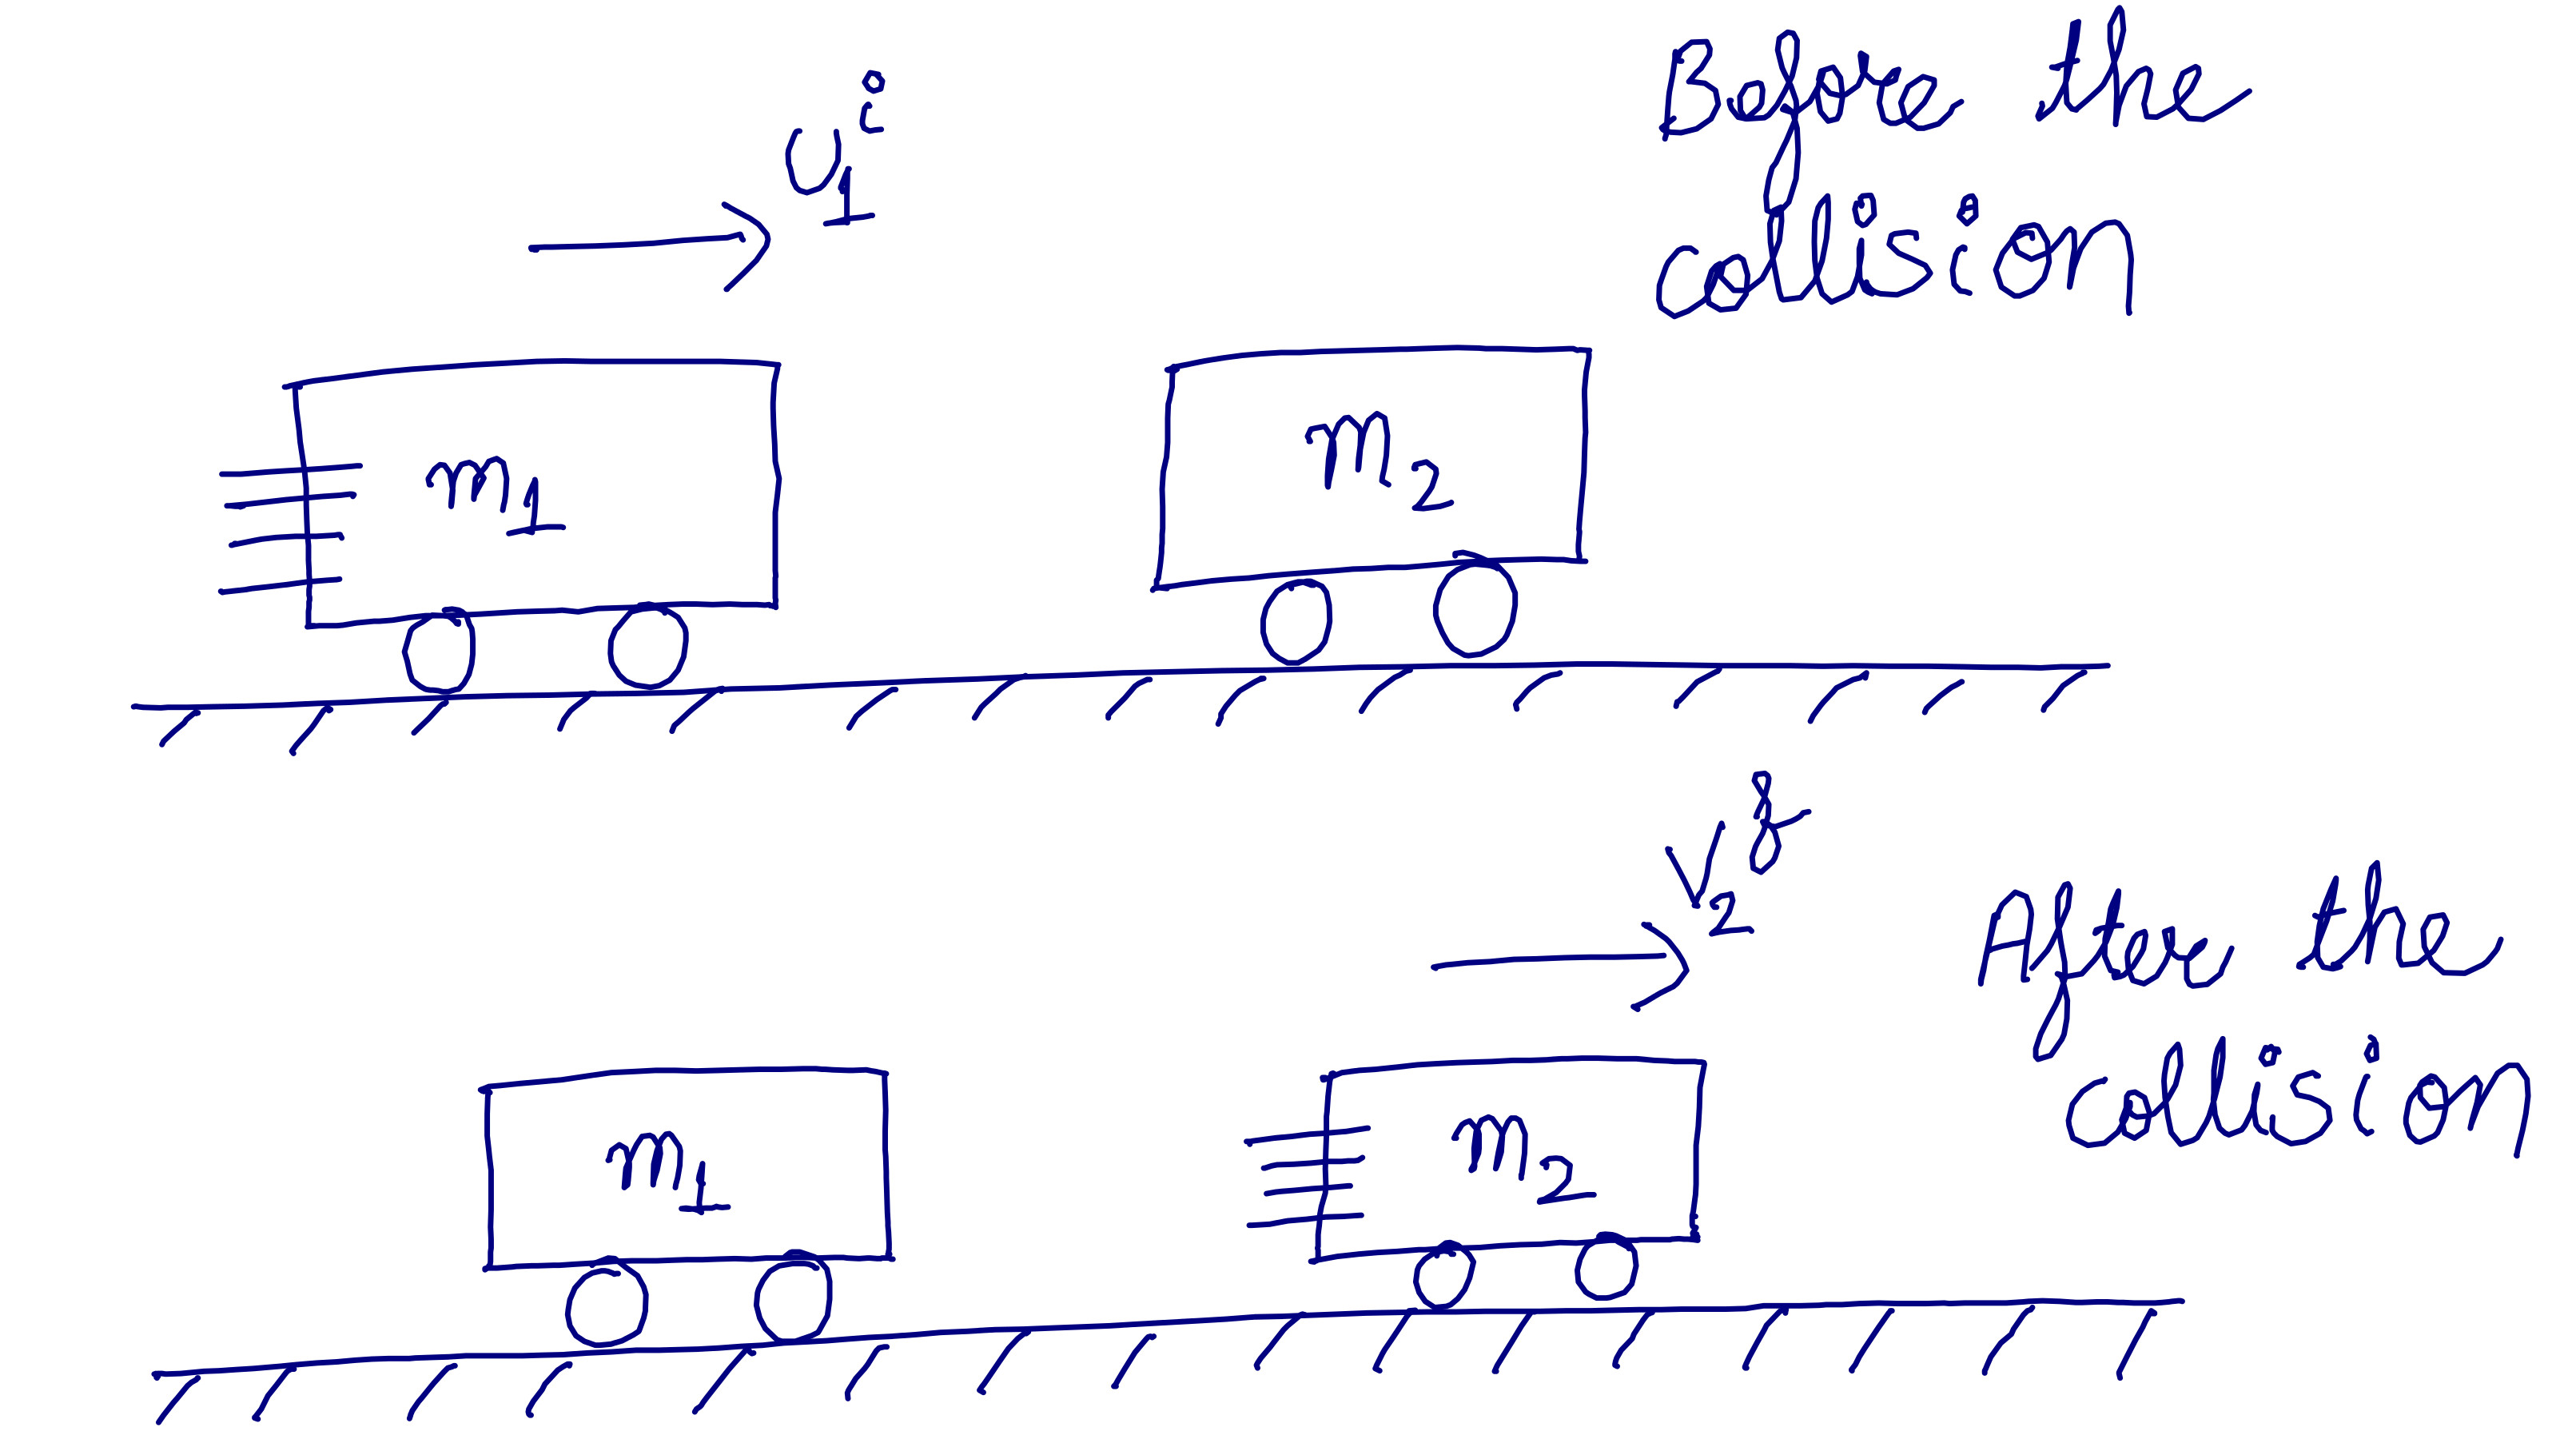
\includegraphics[scale=.4]{collidingmass}
\centering
\caption{Colliding masses}
\label{colmass}
\centering
\end{figure}
Consider the figure \ref{colmass}.  Before the collision, cart 1 had the speed $u_1^i$ and cart 2 was at rest.  It was observed that after the collision, cart 2 gained the speed $v_2^f$ and cart 1 came to rest.

Now we consider the system of two carts as a system with no \emph{net} external force (actually there are two forces which counteract each other).  Thus the conservation of momentum can be applied to the system before and after the collision.  The initial momentum of the system is
\begin{equation}
  p^i_{\text{system}} = m_1u_1^i + m_2\times 0
\end{equation}
and the final momentum is 
\begin{equation}
  p^f_{\text{system}} = m_1\times 0 + m_2v_2^f
\end{equation}
The conservation of momentum implies
\begin{equation}
  p^i_{\text{system}} = p^f_{\text{system}}
\end{equation}
giving the final result
\begin{equation}
  v_2^f = \frac{m_1}{m_2}u_1^i
\end{equation}
\subsection{Rockets}
\begin{figure}[h]
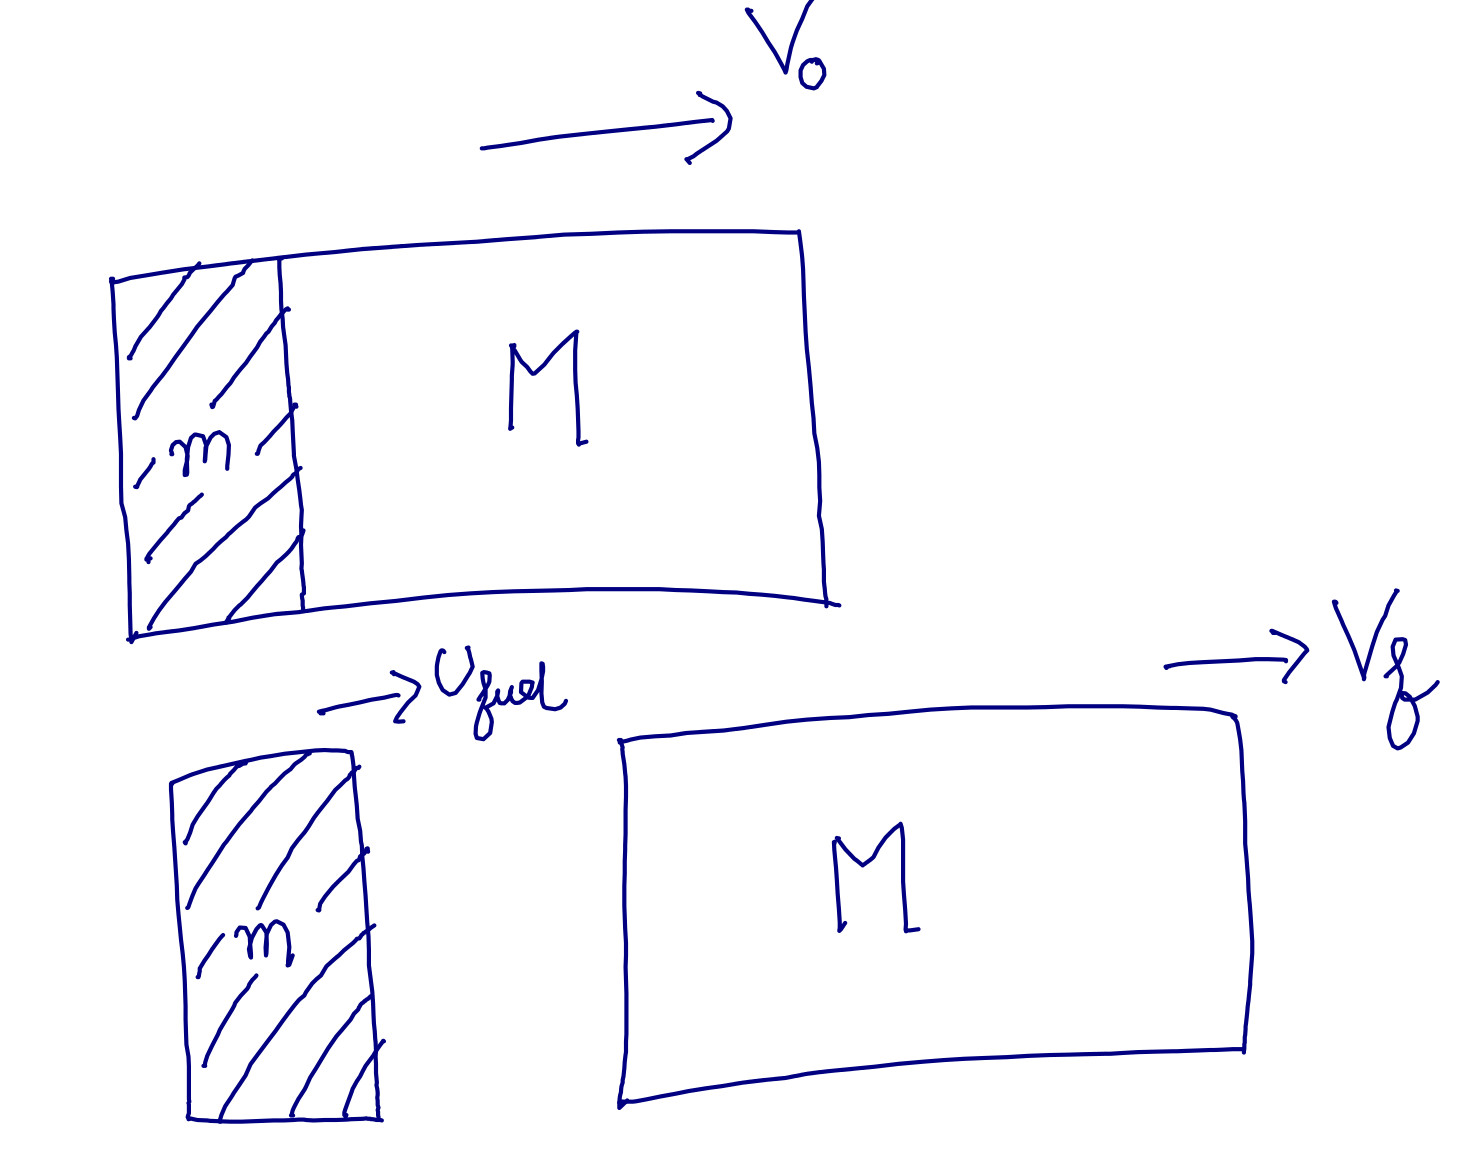
\includegraphics[scale=.4]{rocket}
\centering
\caption{Rocket with fuel}
\label{rockfuel}
\centering
\end{figure}
The working of the rockets can be understood as a consequence of the conservation of the momentum.  Consider the figure \ref{rockfuel}.  The system of the rocket, moving with speed $V_0$, consists of two components.  The fuel component with mass $m_{\text{fuel}}$ and the compartment (where the austronauts sit!) with mass $M$.  Now the rocket ejects the fuel with some speed $u_{\text{fuel}}$ which results in change in the speed of the compartment.
To compute $V_f$, we first write the total initial momentum as
\begin{equation}
  p_{\text{system}}^i=(m+M)V_0
\end{equation}
the final momentum is 
\begin{equation}
  p_{\text{system}}^f=mu_{\text{fuel}}+MV_f
\end{equation}
On equating $p_{\text{system}}^i=p_{\text{system}}^f$ we get the following equation for $V_f$
\begin{equation}
\begin{split}
  V_f &= \frac{(m+M)V_0 - mu_{\text{fuel}}}{M}\\
  &= V_0 + \frac{m}{M}(V_0-u_{\text{fuel}})
\end{split}
\end{equation}
For a ``certain'' condition (you will work out that condition in the sample problems), we see that $V_f>V_0$.  Thus we see as the rocket ejects the fuel, it gains speed and accelerates towards the heavens!
\section{Sample problems}
\begin{enumerate}
\item Consider the collision in figure \ref{colmass}.  Compute the final speed of the cart 2, $v_2^f$ given that $m_1=3$ kg, $m_2=2$ kg and $u_1^i=2$ m/s.
\item In the case of rockets (figure \ref{rockfuel}), find the final speed of the rocket compartment $V_f$ given the initial speed $V_0=30$ m/s, $m=20$ kg, $M=50$ kg and $u_{\text{fuel}}=3$ m/s.  Also \emph{mathematically} state the condition for which $V_f$ is always greater than $V_0$. 
\end{enumerate}
\end{document}
